\documentclass[10pt,a4paper]{article}
\usepackage[UTF8]{ctex}
\usepackage{fontspec}
\usepackage{geometry} 
\usepackage{amsmath}
\usepackage[shortlabels]{enumitem}
\usepackage{float}
\usepackage{graphicx}
\usepackage{subfigure}
\usepackage{epstopdf}


\geometry{left=3.17cm,right=3.17cm,top=2.53cm,bottom=2.54cm}
%\setmainfont{Times New Roman}
\pagestyle{plain}
\setlist[enumerate,1]{label=\textbf{\arabic*.}}
\setlist[enumerate,2]{label=(\arabic*)}
\begin{document}

\begin{enumerate}
    
    \item 写出下列随机试验的样本空间$S$:
    \begin{enumerate}
        \item 记录一个班一次数学考试的平均分数(设以百分制计分).
        \item 生产产品直到有10件正品为止,记录生产产品的总件数.
        \item 对某工厂出厂的产品进行检查,合格的记上“正品”,不合格的记上“次品”,如
        连续查出了2件次品就停止检查,或检查了4件产品就停止检查,记录检查的结果.
        \item 在单位圆内任取一点,记录它的坐标.
    \end{enumerate}



    \item 设$A,B,C$为三个事件,用$A,B,C$的运算关系表示下列各事件:
    \begin{enumerate}
        \item $A$发生,$B$与$C$不发生.
        \item $A$与$B$都发生,而$C$不发生.
        \item $A,B,C$中至少有一个发生.
        \item $A,B,C$都发生.
        \item $A,B,C$都不发生.
        \item $A,B,C$中不多于一个发生.
        \item $A,B,C$中不多于两个发生.
        \item $A,B,C$中至少有两个发生.
    \end{enumerate}



    \item \begin{enumerate}
        \item 设$A,B,C$是三个事件,且$P(A)=P(B)=P(C)=1/4,P(AB)=P(BC)=0,P(AC)=1/8$,
        求$A,B,C$至少有一个发生的概率.
        \item 已知$P(A)=1/2,P(B)=1/3,P(C)=1/5,P(AB)=1/10,P(AC)=1/15,P(BC)=1/20,P(ABC)=1/30$,求
        $A\cup B,\overline{A} \overline{B},A\cup B\cup C,\overline{A}\overline{B}\overline{C},\overline{A}\overline{B}C,\overline{A}\overline{B}\cup C$的概率.
        \item 已知$P(A)=1/2$,(i)若$A,B$互不相容,求$P(A\overline{B})$,
        (ii)若$P(AB)=1/8$,求$P(A\overline{B})$.
    \end{enumerate}


    \item 设$A,B$是两个事件
    \begin{enumerate}
        \item 已知$A\overline{B}=\overline{A}B$,验证$A=B$.
        \item 验证事件$A$和事件$B$恰有一个发生的概率为$P(A)+P(B)-2P(AB)$.
    \end{enumerate}



    \item 10 片药片中有5片是安慰剂.
    \begin{enumerate}
        \item 从中任意抽取5片,求其中至少有2片是安慰剂的概率.
        \item 从中每次取一片,作不放回抽样,求前3次都取到安慰剂的概率.
    \end{enumerate}



    \item 在房间里有10个人,分别佩戴从1号到10号的纪念章,任选3人记录其纪念章的号码.
    \begin{enumerate}
        \item 求最小号码为5的概率.
        \item 求最大号码为5的概率.
    \end{enumerate}



    \item 某油漆公司发出17桶油漆,其中白漆10桶、黑漆4桶、红漆3桶,
    在搬运中所有标签脱落,交货人随意将这些油漆发给顾客。问一个订货为4
    桶白漆、3桶黑漆和2桶红漆的顾客,能按所订颜色如数得到订货的概率是多少?

    
    \item 在1500件产品中有400件次品、1100件正品.任取200件.
    \begin{enumerate}
        \item 求恰有90件次品的概率.
        \item 求至少有2件次品的概率.
    \end{enumerate}



    \item 从5双不同的鞋子中任取4只。问这4只鞋子中至少有两只配成一双的概率是多少?


    \item 在11张卡片上分别写上probability这11个字母,从中任意连抽7张,求其排列结果
    为ability的概率.


    \item 将3只球随机地放入4个杯子中去,求杯子中球的最大个数分别为1,2,3的概率



    \item 50只铆钉随机地取来用在10个部件上,其中有3只铆钉强度太弱。
    每个部件用3只铆钉。若将3只强度太弱的铆钉都装在一个部件上,则这个部件强度就太弱。
    问发生一个部件强度太弱的概率是多少?


    \item 一俱乐部有5名一年级学生,2名二年级学生,3名三年级学生,2名四年级学生.
    \begin{enumerate}
        \item 在其中任选4名学生,求一、二、三、四年级的学生各一名的概率.
        \item 在其中任选5名学生,求一、二、三、四年级的学生均包含在内的概率.
    \end{enumerate}


    \item \begin{enumerate}
        \item 已知$P(\overline{A})=0.3,P(B)=0.4,P(A\overline{B})=0.5$,求条件概率$P(B|A\cup \overline{B})$.
        \item 已知$P(A)=1/4,P(B|A)=1/3,P(A|B)=1/2$,求$P(A\cup B)$.
    \end{enumerate}



    \item 掷两颗骰子,已知两颗骰子点数之和为7,求其中有一颗为1点的概率(用两种方法).


    \item 据以往资料表明,某个三口之家,患某种传染病的概率有以下规律:
    $$P\{\mbox{孩子得病}\}=0.6,P\{\mbox{母亲得病}|\mbox{孩子得病}\}=0.5,P\{\mbox{父亲得病}|\mbox{母亲及孩子得病}\}=0.4$$
    求母亲及孩子得病但父亲未得病的概率.


    \item 已知在10件产品中有2件次品,在其中取两次,每次任取一件,作不放回抽样.求下列事件的概率:
    \begin{enumerate}
        \item 两件都是正品.
        \item 两件都是次品.
        \item 一件是正品,一件是次品.
        \item 第二次取出的是次品.
    \end{enumerate}


    \item 某人忘记了电话号码的最后一个数字,因而他随意地拨号.求他拨号不超过三次而接
    通所需电话的概率.若已知最后一个数字是奇数,那么此概率是多少?


    \item \begin{enumerate}
        \item 设甲袋中装有$n$只白球、$m$只红球;乙袋中装有$N$只白球、$M$只红球。
        今从甲袋中任意取一只球放入乙袋中.再从乙袋中任意取一只球.问取到白球的概率是多少?
        \item 第一只盒子装有5只红球, 4只白球;第二只盒子装有4只红球,5只白球. 
        先从第一盒中任取2只球放入第二盒中去,然后从第二盒中任取一只球.求取到白球的概率.
    \end{enumerate}


    \item 某种产品的商标为“MAXAM” ,其中有2个字母脱落,有人捡起随意放回,求放回后
    仍为“MAXAM”的概率.


    \item 已知男子有5%是色盲患者,女子有0.25%是色盲患者.今从男女人数相等的人群中
    随机地挑选一人,恰好是色盲者,问此人是男性的概率是多少?

    
    \item 一学生接连参加同一课程的两次考试.第一次及格的概率为$p$,若第一次及格则第二
    次及格的概率也为$p$;若第一次不及格则第二次及格的概率为$p/2$.
    \begin{enumerate}
        \item 若至少有一次及格则他能取得某种资格,求他取得该资格的概率.
        \item 若已知他第二次已经及格,求他第一次及格的概率.
    \end{enumerate}




    \item 将两信息分别编码为$A$和$B$传送出去,接收站收到时,$A$被误收作$B$的概率为
    0.02,而$B$被误收作$A$的概率为0.01。信息$A$与信息$B$传送的频繁程度为$2:1$.
    若接收站收到的信息是$A$,问原发信息是$A$的概率是多少?


    \item 有两箱同种类的零件,第一箱装50只,其中10只一等品;第二箱装30只,其中18只
    一等品.今从两箱中任挑出一箱,然后从该箱中取零件两次,每次任取一只,作不放回抽样.求
    \begin{enumerate}
        \item 第一次取到的零件是一等品的概率.
        \item 在第一次取到的零件是一等品的条件下,第二次取到的也是一等品的概率.
    \end{enumerate}


    \item 某人下午5:00下班,他所积累的资料表明:
    
    \begin{table}[h]\centering        
        \begin{tabular*}{\hsize}{cccccc}
        \hline
        \multicolumn{1}{c|}{到家时间}   & $5:35 \sim 5:39$     & $5:40 \sim 5:44$     & $5:45 \sim 5:49$     & $5:50 \sim 5:54$     & 迟于$5:54$             \\ \hline
        \multicolumn{1}{c|}{乘地铁的概率} & 0.10                 & 0.25                 & 0.45                 & 0.15                 & 0.05                 \\ \hline
        \multicolumn{1}{c|}{乘汽车的概率} & 0.30                 & 0.35                 & 0.20                 & 0.10                 & 0.05                 \\ \hline
        \multicolumn{1}{l}{}        & \multicolumn{1}{l}{} & \multicolumn{1}{l}{} & \multicolumn{1}{l}{} & \multicolumn{1}{l}{} & \multicolumn{1}{l}{}
        \end{tabular*}   
    \end{table}
    \vspace{-1cm}
    某日他抛一枚硬币决定乘地铁还是乘汽车,结果他是5:47到家的.试求他是乘地铁回家的概率.


    \item 病树的主人外出,委托邻居浇水.设已知如果不浇水,树死去的概率为0.8.若浇水则
    树死去的概率为0.15.有0.9的把握确定邻居会记得浇水.
    \begin{enumerate}
        \item 求主人回来树还活着的概率.
        \item 若主人回来树已死去,求邻居忘记浇水的概率.
    \end{enumerate}


    \item 设本题涉及的事件均有意义.设$A,B$都是事件.
    \begin{enumerate}
        \item 已知$P(A)>0$,证明$P(AB|A)\geq P(AB|A\cup B)$.
        \item 若$P(A|B)=1$,证明$P(\overline{B}|\overline{A})=1$.
        \item 若设$C$也是事件,且有$P(A|C)\geq P(B|C),P(A|\overline{C})\geq P(B|\overline{C})$,证明$P(A)\geq P(B)$.
    \end{enumerate}



    \item 有两种花籽.发芽率分别为0.8,0.9,从中各取一颗,设各花籽是否发芽相互独立.求
    \begin{enumerate}
        \item 这两颗花籽都能发芽的概率.
        \item 至少有一颗能发芽的概率.
        \item 恰有一颗能发芽的概率.
    \end{enumerate}



    \item 根据报道美国人血型的分布近似地为:A型为37\%,O型为44\%,B型为13\%,AB型
    为6\%.夫妻拥有的血型是相互独立的.
    \begin{enumerate}
        \item B型的人只有输入B、O两种血型才安全.若妻为B型,夫为何种血型未知.求夫是妻
        的安全输血者的概率.
        \item 随机地取一对夫妇,求妻为B型夫为A型的概率.
        \item 随机地取一对夫妇,求其中一人为A型,另一人为B型的概率.
        \item 随机地取一对夫妇,求其中至少有一人是O型的概率.
    \end{enumerate}



    \item \begin{enumerate}
        \item 给出事件$A,B$的例子,使得
        

        (i)$P(A|B)<P(A),\quad$ (ii)$P(A|B)=P(A),\quad$ (iii)$P(A|B)>P(A)$
        \item 设事件$A,B,C$相互独立,证明(i)$C$与$AB$相互独立.(ii)$C$与$A\cup B$相互独立.
        \item 设事件$A$的概率$P(A)=0$,证明对于任意另一事件$B$,有$A,B$相互独立.
        \item 证明事件$A,B$相互独立的充要条件是$P(A|B)=P(A|\overline{B})$.
    \end{enumerate}



    \item 设事件$A,B$的概率均大于零说明以下的叙述(1)必然对,(2)必然错,(3)可能对.
    并说明理由.
    \begin{enumerate}
        \item 若$A$与$B$互不相容,则它们相互独立.
        \item 若$A$与$B$相互独立,则它们互不相容.
        \item $P(A)=P(B)=0.6$ ,且$A,B$互不相容
        \item $P(A)=P(B)=0.6$ ,且$A,B$相互独立.
    \end{enumerate}


    \item 有一种检验艾滋病毒的检验法,其结果有概率0.005报导为假阳性(即不带艾滋病毒
    者,经此检验法有0.005的概率被认为带艾滋病毒).今有140名不带艾滋病毒的正常人全部
    接受此种检验,被报道至少有一人带艾滋病毒的概率为多少?



    \item 盒中有编号为1,2,3,4的4只球,随机地自盒中取一只球,事件$A$为“取得的是1号
    或2号球”,事件$B$为“取得的是1号或3号球”,事件$C$为“取得的是1号或4号球”。验证:
    $$P(AB)=P(A)P(B),P(AC)=P(A)P(C),P(BC)=P(B)P(C),$$
    $$\mbox{但}\quad P(ABC)\neq P(A)P(B)P(C)$$
    即事件$A,B,C$两两独立,但$A,B,C$不是相互独立的。


    \item 试分别求以下两个系统的可靠性:
    \begin{enumerate}
        \item 设有4个独立工作的元件1,2,3,4.它们的可靠性分别为$p_1,p_2,p_3,p_4$,将它们按
        图(1)的方式连接(称为并串联系统).
        \item 设有5个独立工作的元件1,2,3,4,5.它们的可靠性均为$p$,将它们按图(2)的
        方式连接(称为桥式系统).
        \begin{figure}[H]
        \centering
        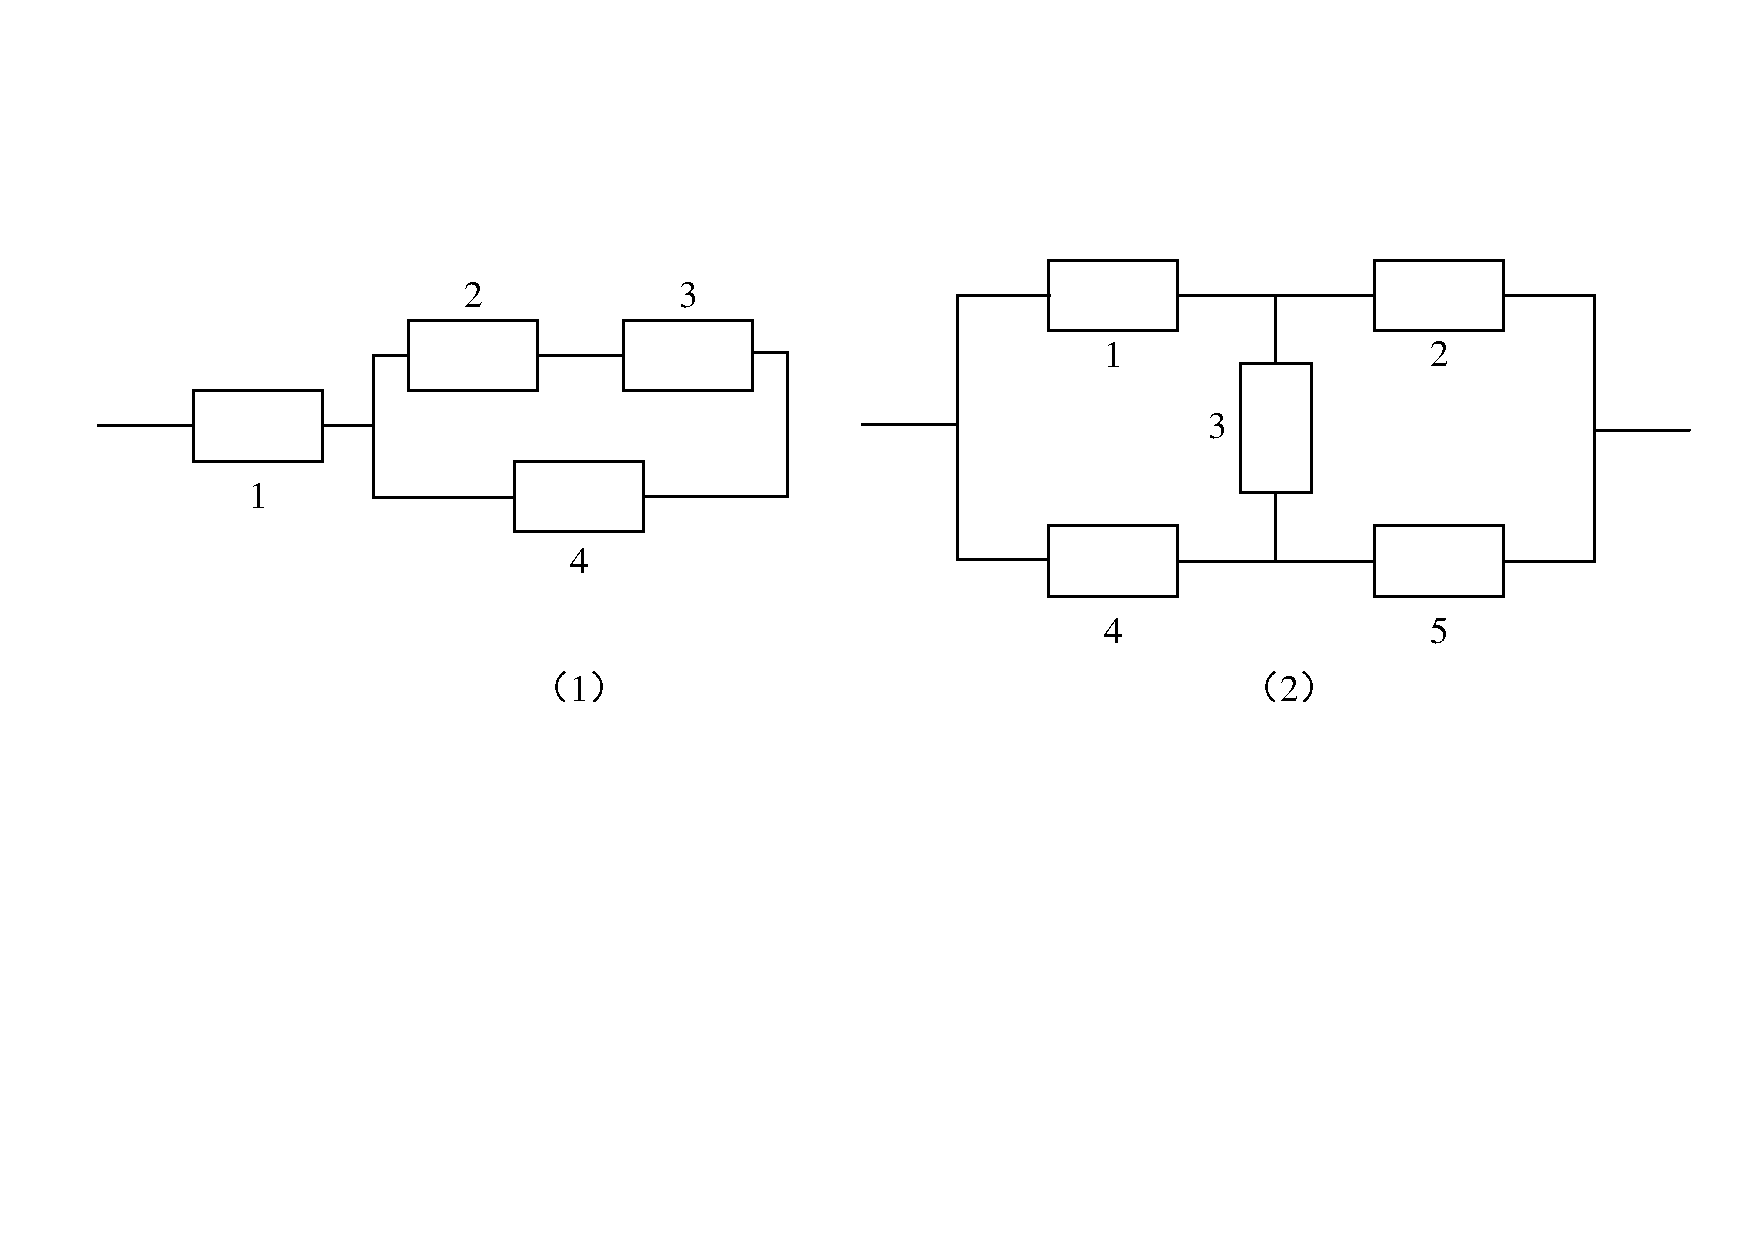
\includegraphics[width=0.8\textwidth]{1.34.pdf}
        \end{figure}
        \vspace{-0.5cm}
    \end{enumerate}



    \item 如果一危险情况$C$发生时,一电路闭合并发出警报,我们可以借用两个或多个开关
    并联以改善可靠性.在$C$发生时这些开关每一个都应闭合,且若至少一个开关闭合了,警报
    就发出. 如果两个这样的开关并联连接,它们每个具有0.96的可靠性(即在情况$C$发生时闭
    合的概率),问这时系统的可靠性(即电路闭合的概率)是多少?如果需要有一个可靠性至少
    为0.9999的系统,则至少需要用多少只开关并联?设各开关闭合与否是相互独立的.


    \item 三人独立地去破译一份密码,已知各人能译出的概率分别为$1/5,1/3,1/4$. 问三人
    中至少有一人能将此密码译出的概率是多少?


    \item 设第一只盒子中装有3只蓝球,2只绿球,2只白球;第二只盒子中装有2只蓝球,3
    只绿球,4只白球.独立地分别在两只盒子中各取一只球.
    \begin{enumerate}
        \item 求至少有一只蓝球的概率.
        \item 求有一只蓝球一只白球的概率.
        \item 已知至少有一只蓝球,求有一只蓝球一只白球的概率.
    \end{enumerate}


    \item 袋中装有$m$枚正品硬币、$n$枚次品硬币(次品硬币的两面均印有国徽),在袋中任取一
    枚,将它投掷$r$次,已知每次都得到国徽.问这枚硬币是正品的概率为多少?


    \item 设根据以往记录的数据分析,某船只运输的某种物品损坏的情况共有三种:损坏2\%
    (这一事件记为$A_1$) ,损坏10\%(事件$A_2$),损坏90\% (事件$A_3$) ,且知
    $P(A_1)=0.8,P(A_2)=0.15,P(A_3)=0.05$现在从已被运输的物品中随机地取3
    件.发现这3件都是好的(这一事件记为$B$).试求$P(A_1|B),P(A_2|B),P(A_3|B)$
     (这里设物品件数很多,取出一件后不影响取后一件是否为好品的概率).


     \item 将$A,B,C$三个字母之一输入信道,输出为原字母的概率为$\alpha$,而输出为其他一字母
     的概率都是$(1-\alpha)/2$.今将字母串AAAA,BBBB,CCCC之一输入信道,输入AAAA,BBBB,
     CCCC的概率分别为$p_1,p_2,p_3(p_1+p_2+p_3=1)$,已知输出为ABCA,问输入的是AAAA的
     概率是多少?(设信道传输各个字母的工作是相互独立的.)

\end{enumerate}
\end{document}